
\documentclass[11pt,a4paper]{report}
\usepackage[utf8]{inputenc}
\usepackage{graphicx}
\usepackage{multicol}
\usepackage{hyperref}
\hypersetup{
    colorlinks=true,
    linkcolor=blue,
    filecolor=magenta,      
    urlcolor=blue,
}
\usepackage[left=2cm,right=2cm,top=2cm,bottom=2cm]{geometry}
\author{C.A.Valliappan}
\title{Signal detection and decoding for ADSB}
\begin{document}
\chapter{GSoC Proposal 2017 - AerospaceResearch.net}

\textbf{Project Title }: Signal detection and decoding for ADSB\\
\textbf{Name}: Valliappan\\
\textbf{Degree}: B.E(Hons) Electronics and Instrumentation\\
\textbf{University }: Birla Institute of Technology and Science-Pilani, India\\
\textbf{Location/Timezone}: India, GMT +5:30\\ 
\textbf{Mentor}: Andrews Hornig \& Muzy\\

\section{Introduction}
On 1090 MHz airplanes are transmitting their meta data like aircraft id, location, speed and direction.It is called adsb. I have to create A Module out of the python libdump1090. The module needs to be loadable by the ground station main software. The output shall be each adsb signals by their data and the starting time (sample count) within the input file (an iq-stream).

\subsection{Main features of libdump1090}
1.Robustness in decoding the weak messages.\\
2.Single bit error correction.\\ 
3.Pre-calculated checksum table for D11 and D17.\\
4.This libdump1090 can decode DF0, DF4, DF5, DF16, DF20 and DF21 where the checksum is xored with the ICAO address by brute forcing the checksum field using recently seen ICAO addresses.

\subsection{Limitations}

1)The libdump1090 works fine only if the data is less than or equal to 1024Kb.\\ 2)The main code is written in C and python wrapper to exicute in python. Instead of uniform python module. Hence making it two language dependent.\\
3)Mode\_s.c code uses huge amount of precomputed values. For example the magnitude lookup table which has a size of 65536.\\
4)The output of the ADSB decoded message is not compact, as it displays the unwanted parameters corresponding to the Dataframe number. 

\section{Project Goals}
 
I would also like to incorporated some changes to the main code:-
\begin{itemize}
\item Primary objective of the project is to make the code work for input file size greater than 1Mb.
  \item Return a new aircraft structure for the interactive mode.
  \item CPR coordinates decoding and track calculation from velocity using manual[5]
  \item Display of the compact decoded message consisting of only the essential parameter corresponding to the Dataframe. The output shall be time, ADSB signal and the decoded message.    
\end{itemize}
Intergrating changes to ground station main software. Hence making a working model ready for Distributed Ground Station Network.\\

Simultaneously, I would like to implement the Mode\_s decoding algorithm from scratch as a python module. I would handle this by implenting each block and testing their work and proceeding to the next block as shown in \textbf{Figure 1.1} . There is already an academic implementation available in C [1], but it is not well-supported with the python wrapper.      
\begin{figure}[h]
\centering
\includegraphics[scale=0.5]{1}
\caption{Flowchart based on the understanding of libdump1090 code  }
\end{figure}
\section{Implementation}
I will be discussing the implemention procedure for each of my project goals discussed above:- \\
1)Making the code working good for any input file size. Here are variables, that has created possible problem in the earlier code.
\begin{verbatim}
    MODES_ASYNC_BUF_SIZE = 4*16*16384 \\ 1Mb  defined in Mode_s.c
    ADSB_BUF_SIZE = 4*16*16384 # 1MB defined in Mode_s.py
\end{verbatim}
Initially, I used the pincipal of divide and conquer, where I will divide the big file into many small 1Mb files. If the file is less than 1Mb then remaining values will be appended with 1's.
\href{https://github.com/PRRvalli/libdump1090/blob/master/new_modes.py}{Link to the code}. This idea was adopted from \href{https://github.com/antirez/dump1090}{[1]} where
\begin{verbatim}
   MODES_DATA_LEN = 16*16384. \\ 256Kb
   \\ Each time the buffer is filled with 256Kb of data and used for decoding
   \\ It goes on reading till end of the file. 
   \\ If the buffer doesn't have sufficient data, then the rest of the data will be
   \\ filled with 1's.   
\end{verbatim}
The output of \textbf{Mode\_s.py} program should display the decoded message  as compact as follows: 
\begin{verbatim}
   Message : 8d3c6dd358b980a9ee026ce0c7eb;
   CRC: 000000 (ok)
   DF 17: ADS-B message.
      Capability     : 5 (Level 2+3+4 (DF0,4,5,11,20,21,24,code7 - is airborne))
      ICAO Address   : 3c6dd3
      Extended Squitter  Type: 11
      Extended Squitter  Sub : 0
      Extended Squitter  Name: Airborne Position (Baro Altitude)
      F flag   : even
      T flag   : non-UTC
      Altitude : 36000 feet
      Latitude : 21751 (not decoded)
      Longitude: 620 (not decoded)

\end{verbatim}
This can be done by adding if-else statements in \textbf{\texttt{displayModesMessage()}} function.\\

The final part of the project would the implementation of python module from the scratch. I would like to make an approach to this implementation systematically as shown in the block diagram \textbf{Figure 1.2}.    
\begin{figure}[h]

\includegraphics[scale=0.6]{implement}
\caption{Implementation work Flow}
\end{figure}
\\
\\
For the implementation I will write many helper functions and their purpose are self explanatory from the function names. The function list is rough sketch based on the requirements. The structures defined in the mode\_s.c will be converted implemented as class in the new python implementation which improves the security of the information. \\
The Function list for \textbf{RawIQ to message}:
\begin{figure}[h]
\centering
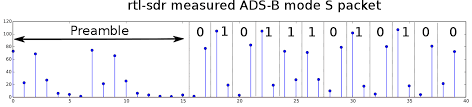
\includegraphics[width=12cm,height=2.5cm]{images}
\caption{Preamble \& Payload}
\end{figure}
\begin{verbatim}
computeMagnitudeVector(IQ_Data) # this function uses the magnitude lookup table

decodemodeS(magnitude_vector)
Iterate through the magnitude vector check for a valid Preamble of 16 bits as 
shown in figure (1.3). 
   |--> first check for consecutive 10 samples representing a valid preamble.
   |--> The samples between the two spikes must be < than the average 
        of the high spikes level.
   |--> Similarly samples in the range 11-14 must be low.

If the above attempt with this message failed retry with Phase_correction()  

If the proper preamble is found then we will decode the message length based on 
conditions implemented by muzy
   |--> Here we would like to cross check if the message length found from 
        dataframe is same as the message length detected.
   |--> Finaly before decoding message we check for Signal strength > 0x02FF and 
        Errors <= 3.  
   |--> Decode the message using decodeModesMessage(message).
   |--> update the iterate pointer to 'preamble_size + message_len'     

If you cannot find the message retry with phase correction.

Phase correction Function:

detectOutOfPhase(Preamble) 
# Return -1 if the message is out of phase left-side
# Return  1 if the message is out of phase right-size
# Return  0 if the message is not particularly out of phase.

clamped_scale(value, scale)
#returns a scaled valued <= 65535 , this function is used in PhaseCorrection()

PhaseCorrection(magnitude_vector[preamble+paylode])
#Algorithm is same as libdump1090 code written by muzy.
\end{verbatim} 
\textbf{Error Correction will be the next major task which is implemented similar to libdump1090 code:}
\begin{verbatim}
Pre-Defined modes_checksum_table of size 112 each 32bit hexadecimal value

modesChecksum(message, msg_len)  #Returns 24 bit checksum syndrome.

modesInitErrorInfo()   
# Compute the table of all syndromes for 1-bit and 2-bit 
# error vectors making it less intensive for the computer


fixBitErrors(message, bits_to_fix)
# Search for syndrome in table and if an entry is found, flip the necessary
# bits. Make sure the indices fit into the array
\end{verbatim} 
\textbf{Lastly decoding the message:}
\begin{verbatim}
decodeModesMessage(message)
Decode message type DF0, DF4, DF5, D11, DF16, D17, DF20 and DF21.
With special emphasis on DF20 and DF21
Mode S Enhanced Surveillance (EHS)
Downlink Format and message structure
    Parity and ICAO address recovery
    Address Parity
    BDS (Comm-B Data Selector), BDS 2,0 (Aircraft identification), BDS 4,0 
    (Selected aircraft intention)
    BDS 4,4 (Meteorological routine air report), BDS 5,0 (Track and turn report),  
    BDS 6,0 (Heading and speed report)
    as illustrated in [2]
Lastly CPR coordinates decoding and track calculation from velocity based on[2 & 5].
interactiveShowData()
   Interactive Display of aircraft information with CPR latitude and longitude .	
    
ICAOCacheHashAddress(address)
# if crc == 0 try to populate our ICAO addresses whitelist.

addRecentlySeenICAOAddr(address)
# if crc == 0 try to populate our ICAO addresses whitelist.

ICAOAddressWasRecentlySeen(address)
# Compare the checksum with the whitelist of recently seen ICAO
# addresses. If it matches one, then declare the message as valid
\end{verbatim}


\section{Timeline}

\textbf{Community Bonding Period}
\begin{itemize}
\item A huge part of being part of the open-source community and Google Summer of Code is sharing your ideas and work. I've started a blog \href{https://valliappanca.wordpress.com/}{here} to give weekly reports of the summer work I will be doing, and try and break down the world of probabilistic topic models to everyone.
\item Before the official time period begins I intend to fix the issue of libdump1090's failure for input file size $> $ 1Mb. Along with the displayModesMessage() for displaying compact Mode\_s message.  


\end{itemize}
\textbf{Week 1:}
\begin{itemize}
\item Start with the Python implementation of decoding Raw IQ data to magnitude vector.
\item Testing is done use the pre-existing \textbf{output.bin} and \textbf{IQ\_data.dat} given by Andreas during the discussion period.
\item Last 2 days of the this week is alloted for backup and documentation.    
\end{itemize} 
\textbf{Week 2 and 3:}
\begin{itemize}
\item Decoding Modes from the magnitude vector by checking for preamble 
\item Phase correction, Signal Strength check \& Error check $<$ 3 
\item Ultimately detect the message length .
\item Testing and documentation
   
\end{itemize} 
\textbf{Week 4 and 5:}
\begin{itemize}
\item Cyclic Redundancy check and Check sum implementation 
\item Bit error correction 
\item Implementing error correction important step. Hence to be handled with intensive care.
\item Testing and documentation and update the blog.
   
\end{itemize} 
\textbf{\\Week 6 to 7:}
\begin{itemize}
\item Decoding the Mode\_s message based on the manual [2,3 \& 5] 
%\item Bit error correction 
%\item Implementing error correction important step. Hence to be handled with intensive care.
\item Keep working on the blog as well!
   
\end{itemize} 
\textbf{Final Phase :}
\begin{itemize}
\item Integrating the changes to DGSN  
\item Making requirement changes that the above implementation can also be used for data recieved from Software Defined Radio (RTL-SDR).   
\item Signal ADSB Visualisation in the interactive manner. based on interactiveShowData()[1,4 \& 5]. 
\item Keep working on the blog as well!
   
\end{itemize} 
\section{Furture work}
Apply other kind of Correction for magnitude vector as discussed in paper [6,7], to investigate improved squitter reception techniques. For more capable error correction algorithms, and more selective preamble detection.
\section{Commitments}
My next summer vacation starts by May $10{^th}$ and next semester course work begins by August $2^{nd} $ week. Hence I will not be occupied with any other work during the GSoC Program and will dedicate my full concentration on project. \\
I would take Sundays off but will maintain a minimum of 40Hrs per week.If required by mentors, I will make required changes to my proposal. Also, I have not applied for any other organisation. 

  
\section{Reference}

[1]\href{https://github.com/antirez/dump1090}{Dump1090 written by Salvatore Sanfilippo.}
[2]\href{http://adsb-decode-guide.readthedocs.io/en/latest/}{ADSB-decoding guide}
[3]\href{https://www.ll.mit.edu/mission/aviation/publications/publication-files/atc-reports/Gertz_1984_ATC-117_WW-15318.pdf}{Mode\_s Implementation manual by Lincoln Laboratory}
[4]\href{https://github.com/MalcolmRobb/dump1090}{MalcoRobbs Dump1090 implementation.} 
[5]\href{http://www.lll.lu/~edward/edward/adsb/DecodingADSBposition.html}{http://www.lll.lu/~edward/edward/adsb/DecodingADSBposition.html\\}
[6]Barhydt, Richard, et al. "ADS-B within a multi-aircraft simulation for distributed air-ground traffic management." Digital Avionics Systems Conference, 2004. DASC 04. The 23rd. Vol. 1. IEEE, 2004.\\
7]Harman, W., J. Gertz, and A. Kaminsky. "Techniques for improved reception of 1090 MHz ADS-B signals." Digital Avionics Systems Conference, 1998. Proceedings., 17th DASC. The AIAA/IEEE/SAE. Vol. 2. IEEE, 1998.
\section{Contacts}
\textbf{Facebook} :\href{https://www.facebook.com/valliappan.ca}{Valliappan CA}\\
\textbf{Twitter }:\href{https://twitter.com/valliappanca}{@valliappanca}\\
\textbf{Gmail \& Gtalk }:spmanikam@gmail.com\\
\textbf{Skype }:valliappan.ca\\
\textbf{Github Handle} : \href{https://github.com/PRRvalli}{PRRvalli}\\
\href{https://valliappanca.wordpress.com/}{Blog related to my GSoC Project}\\
\textbf{Phone \& Whatsapp} : +91-8378988093 \\
\textbf{Github Repository } :\href{https://github.com/PRRvalli?tab=repositories}{Project that I coded}\\
\textbf{Google drive} : \href{https://drive.google.com/drive/folders/0B70247lHo_0NVkN1UUdVZklfaTg?usp=sharing}{Link}
\chapter{Motivation Letter}
Being an undergraduate student for me studies is all about exploring new fields of science. Through out my undergraduate studies I have worked with many signals, starting from bio-medical signals like brain signals(EEG), Speech signals, ECG etc. I have also worked on artificial signals like Broadband reflectometry signal, this gave me the first experience working with IQ data. Every signal has information embedded in them as engineers my duty is to study them to decode the information. So far I have been success full in doing so with the above mention signal. My github projects and CV is evidence for my knowledge in this field.\\

My academic courses on Satellite communication, Mobile telecomunication network \& Telecom-Switching Network has enriched me with the required knowledge for understanding the idea \textbf{"Signal Detection and Decoding of ADSB"}. I'm an active code in hackerrank and SPoJ as I'm interest towards Data Structures and Algorithm. My prefered languages are C/C++, Python and Matlab. I prefer Matlab for visualisation of data graphically. Hence I think I am very well suited to work on the proposed project imlementation as it required good comfort level in Python and C++ along with algorithm to implement efficiently. \\

Every Single project ideas proposed in AerospaceResearch.net organisation are interesting and enthusiatic especially because of the wonderful visuals especially "\textbf{Lone Pseudoranger}" project for data visualisation. This bring celestial objects close to us, that excites me. Being an Electronics and Instrumentation student, and my deep interest with signal made me choose the project idea  \textbf{"Signal Detection and Decoding of ADSB"}. Added to this AerospaceResearch.net organisation has wonderful mentor Mr.Andreas who has be patiently answering my doubts from the start. I have learned a lot of essential information from him and I'm highly motivated to work with him during the summer 2017 by contributing for GSoC project. 

  

            

\end{document}